\section{Introduction}\label{sec::introduction}

The precise measurement of the angle \g of the Cabibbo-Kobayashi-Maskawa (CKM) unitarity triangle is on the top of the flavour physics program of \lhcb experiments. The CKM angle \g is one of the least well-determined CKM parameters and may be extracted using time-independent rates of decays such as \Bp\to\Dzb\Kp or by the time-dependent study of the \Bs\to $D_s^{(*)\pm}$\Kmp decays or the analogous \Bs\to $D_s^{(*\pm)}$\pimp. In the time-dependent measurements with the family of $B_{s,d}$\to$D_{s,d}h$ decays the sensitivity to results from the interference between the \bquark\quarkbar\to(\cquark\quarkbar)(\uquarkbar\quark) and \bquark\quarkbar\to(\uquark\quarkbar)(\cquarkbar\quark) transitions that occurs through the \Bz\Bzb and \Bs\Bsb mixing.

Determination of the CKM angle \g in tree-level open-charm b-hadron decays are theoretically clean. It is a good opportunity to measure sensitive to New Physics beyond the Standard Model effects. The precision obtained at \lhcb experiment allows the angle \g to be determined with an uncertainty of around 5$\degree$. This precision is obtained by combining various measurements performed at \lhcb  as the most accurate measurements have an accuracy of 10$\degree$ to 20$\degree$. 

The analysis of  \Bs\to\Dss\KS\pim and \Bs\to\Dss\Kstarm decay is believed to be challenging because it requires the selection of soft photon from \Dss\to\Ds\g and (\Bs\to\Dss\Kstarm analysis) reconstruction of resonance state \Kstarm which decay to \KS and another pion. Since the \KS mesons are reconstructed at \lhcb using a different type of track, the selection of candidates is divided to events with \KS reconstructed using downstream and long track respectively. The \Ds meson is reconstructed only \Dss\to\Km\Kp\pip mode.

This decay has not been observed before. In this note, we describe the reconstruction of, \Bs\to\Dss\Kstarm, \Bs\to\Dss\KS\pim and XXXX using the full Run 2 data sample. The XXXX has already been observed, and its branching fraction is. Here we report the first observation of \Bs~\to\Dss\KS\pim and \Bs~\to\Dss\Kstarm. This is the first step towards of the future measurement of time-dependent CP asymmetry in \Bs~\to\Dss\Kstarm decay.

\begin{figure}[h]
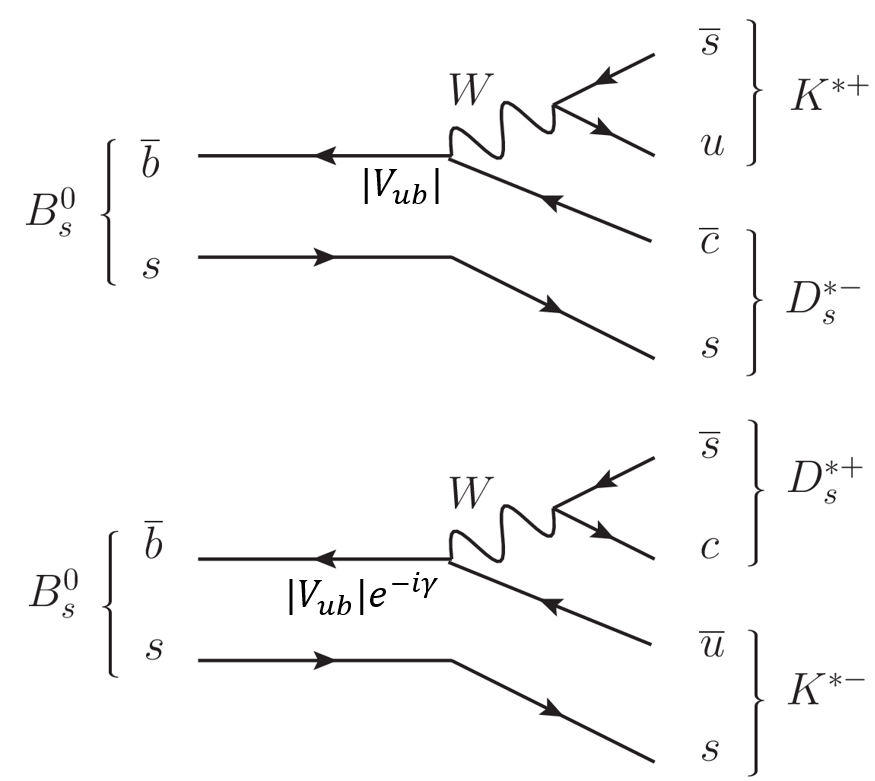
\includegraphics[width=9cm]{figs/feynman_diagram.png}
\centering
\caption{Feynman diagram for \Bs\to\Dss\Kstarm decay. }
\label{fig:feymnan}
\end{figure}

